\documentclass[a4]{report}
\def\atitle{Rheometor Control System: Hardware Overview}
\def\theauthor{Christopher Boyle}
\def\thewords{4466}

\def\br{\newline \newline \noindent}
\def\cbh{\large\bfseries !!! ??? !!! \normalsize\normalfont}

% Imports
\usepackage{graphicx}
\usepackage[a4paper]{geometry}
\usepackage{fancyhdr}
\usepackage[english]{babel}
\usepackage{etoolbox}
\usepackage{url}
\usepackage[hidelinks]{hyperref}
\usepackage{subcaption}

% Unused packages
%\usepackage{placeins}
%\usepackage{fancyref}
%\usepackage[comma,authoryear]{natbib}
%\usepackage{lipsum}

% Settings
\geometry{top=2cm, bottom=2.5cm, left=3cm, right=2.5cm}
\patchcmd{\chapter}{\thispagestyle{plain}}{\thispagestyle{plain}}{}{}
\patchcmd{\section}{\thispagestyle{plain}}{\thispagestyle{plain}}{}{}
\patchcmd{\subsection}{\thispagestyle{plain}}{\thispagestyle{plain}}{}{}
\setcounter{secnumdepth}{0}
\renewcommand{\theequation}{\arabic{equation}}
\renewcommand\UrlFont{\rmfamily\itshape}
\setlength{\fboxsep}{0pt}
\setlength{\fboxrule}{0pt}
\def\achapter{preamble}
%%%% TEMPLATES
\iffalse


%%%EQUATION

	\begin{equation}
		(THE EQUATION)
		\label{EQUATION REF}
	\end{equation}


%%%FIGURE

	\begin{figure}[!htb]
		\centering
		\fbox{\includegraphics[scale=SCALE]{IMAGE LOCATION}}
		\caption{CAPTION}
		\label{FIGURE REF}
	\end{figure} \newline  \noindent

%%%BULLET POINT LIST
	\begin{itemize}
	\item
	\end{itemize}

\fi
%%%%

% Header/footer preamble
\fancyhf{}
\fancypagestyle{plain}{
	\renewcommand{\headrulewidth}{0.4pt}
	\renewcommand{\footrulewidth}{0.4pt}
%	\fancyhead[L]{\atitle}
	\fancyhead[L]{\achapter}
	\fancyhead[R]{\theauthor}
	\fancyfoot[L]{\today}
	\fancyfoot[R]{\thepage}
}
\pagestyle{plain}

\begin{document}
%%%%%%%%%%%%%%%%%%%%%%%%%% TITLE PAGE
	\begin{titlepage}
		\makebox[\textwidth][c]{
\includegraphics[scale=1]{images/titleheader.png}}
		\centering
		\vskip4cm
		{
			\bfseries\Large
			Department of Chemical \& Process Engineering\\
			\vskip1cm
			MEng in Chemical \& Process Engineering\\
			18530
			\vskip3cm
			\LARGE\atitle
		}
		\vskip3cm
		\begin{flushleft}
			\vskip3cm
			Your name: \theauthor \hfill Date: \today
			\vskip1cm
			Organisation: University of Strathclyde, Department of Chemical \& Process Engineering\newline% \newline
			In-house Supervisor: Dr. Leo Lue \newline% \newline
			Academic Supervisor:  Dr. Leo Lue
		\end{flushleft}
	\end{titlepage}
	
	% Contents Page
	\def\achapter{Contents}
	\tableofcontents
	
	\pagenumbering{arabic}
	\setcounter{page}{1}
	
%=====------++++++=====------++++++=====------++++++=====------++++++=====------++++++=====------++++++=====------++++++=====------++++++=====------++++++=====------++++++=====------++++++=====------++++++=====------++++++=====------++++++=====------++++++=====------++++++
                                                               
	\chapter{Introduction}
	


\section{Laboratory Automation and Process Control}
%summ back mot, struct, conc
Laboratory automation involves the design and implementation of robotic systems which are able to conduct laboratory experiments automatically, reducing the workload of human scientists and technicians \cite{backwhatisauto}. This includes the use of machine learning and AI to interpret results and create hypotheses \cite{backlitrevai, backbaconauto, backlabauto}. The motivation for this is eaasy to see, "Robot Scientists" can be used to conduct experiments with little to no human supervision and can take in a vast number of measurements. The "Adam" Robot Scientist developed by the team at Aberystwyth University can make over 1,000,000 observations and hypotheses per day \cite{backontorobsci}. \cbh %safety? toxic environs?
\br
Laboratory automation emerged in the late 19th century, with siphons and controlled flow of water used to automate various processes. As technology advanced and electronics became more prevalent, the options for automation in the laboratory increased. Automatic titration equipment (using photo-cells to detect a colour change) were revolutionary in their ability to accurately and consistently record results, especially for difficult to discern colour changes \cite{backlabautohisto}. \br
Process control can be thought of as the industrial mirror of laboratory automation which has developed along a similar path starting with mechanical analogue device, moving into electronically assisted technology and then, with the advent of computer technology, process control became the marriage of digital and analogue systems it is today \cite{backautocontrolhisto}.
Process control is an inherent area of process design; the process (whatever it may be) has parameters which must be controlled so that the process continues under the design paramters; at the correct temperature, pressure, etc. Process control has historically been achieved through the use of analogue equipment, using pressurised air to send and receive signals from process equipment. Modern process control is achieved through the use of computers and digital electronics, where the analogue measured signals are converted into digital signals, so that a computer can understand the data. The controller applies an algorithm to calculate the control action required to maintain the desired value of the variable. The modern digital controller can deal with almost any form of input, guarding against a wide variety of disturbances. If it can be measured, it can be controlled.\br
At the heart of the modern controller is the control algorithm. This is the calculation which determines what change to the control output needs to be made (the control action). Control algorithms vary with application. The most commonly used algorithm is the Proportional-Integral-Derivative algorithm (PID control), consisting of three sections which can be turned off or on depending on the needs of the situation:
\begin{itemize}
	\item Proportional control increases the control action proportional to the size of the error (the difference between the set point and the measured value). This is easy to tune and set up, however it suffers from offset bias. This bias arise from the control action being balanced out in the process by the error such that the control action is not sufficient to change the process to compensate for the error. The error will remain, and the controller will do no more to correct for it, thus an offset is sustained. This must be manually corrected for.
	\item Integral control increases the control action depending on the integral of the error with respect to time (the longer the error goes on, the higher the control action). Integral action is useful to eliminate the offset bias of proportional control.
	\item Finally, derivative control increases control action with the derivative of the error with respect to time, so a quickly rising error is met with a large change in control action. Derivative action is difficult to tune and highly sensitive to noise in the circuit - this means it is rarely used. If it is used, it requires some form of noise filter on the signal and careful tuning. The most common version of the PID algorithm only uses proportional and integral action (no derivative) - the PI controller. PI control allows for easy tuning and quick response, without the difficulties of derivative action, or the offset bias of proportional control.
\end{itemize}
Each control element has an associated gain parameter which affects how strongly that element is represented in the control action. These parameters must be set properly before controller can be used. This is done in a process called tuning. There are a variety of methods for tuning the controller, most commonly used is the Ziegler-Nichols method, involving tuning the controller such that the measured value oscillates in a sustained way. Then using the period of oscillation along with other measured parameters to decide on the optimum controller tuning. After tuning using a method such as Ziegler-Nichols it is often required to tweak the tuning manually to obtain the most effective controller for the situation. This is done mostly by trial and error. Trial and error tuning can also be used to fully tune the device, although this would take a long time to do by hand. \br
The controller device itself is a small computer, reading input from the instruments and then applying the algorithm to determine how it should alter the process. These small computers are called "microcontrollers". A microcontroller chip is a small re-programmable computer which reads input from, and outputs data to an electronic circuit \cite{backwhatismc}. Microcontrollers are programmed by connecting them to a "master" computer which can set the data on the microcontroller's storage. Data is stored as binary data (data is stored solely in the form of 0s and 1s). The program is written in a programming language, a special set of instructions which the environment can understand and convert into actions. \br

%	\begin{figure}[h!]
%	\centering
%	\fbox{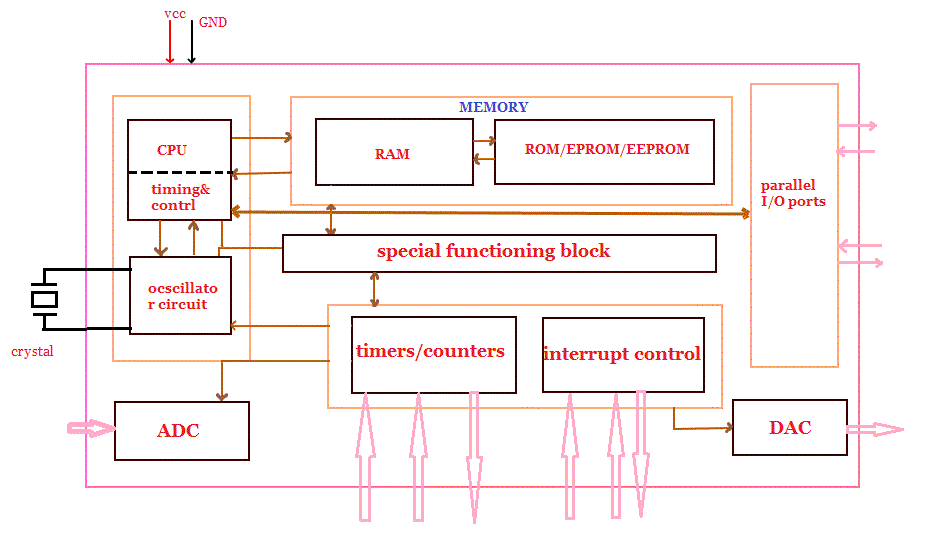
\includegraphics[scale=0.5]{images/mcudia.png}}	\caption{Microcontroller Block Diagram (taken from  \cite{mcudia})}
%	\label{mcudia}
%	\end{figure}




\section{Raspberry Pi} % section last edited 3/3/2017
\noindent
Microcontrollers are commonly used in education to teach computer programming \cite{backmcedu1, backmcedu2}. However, it was noticed that people were not properly learning about how computers work in schools and universities and so a team of academics at the University of Cambridge created the Raspberry Pi Foundation, and developed the Raspberry Pi Model A as a platform to facilitate education \cite{pihistory}. The Raspberry Pi is a small (85mm x 56mm \cite{pi3mechdraw}) computer. By default, it runs a version of GNU/Linux called "Raspian". There are a number of alternative operating systems suitable for different applications (media center, embedded smart technology) \cite{piotheros}.  \newline
\begin{figure}[!htb]
	\centering
	\fbox{\includegraphics[scale=0.3]{images/annotpidia.png}} %https://www.draw.io/#Hcbosoft%2Fpi_rheo_proj%2Fmaster%2Fwrite_up%2Fimages%2Fannot_pi_dia.xml
	\caption{Raspberry Pi 3 Model B (adapted from  \cite{pi3info})}
	\label{pidia}
\end{figure} \newline% \noindent
The first Raspberry Pi (Model A) had a single core 700MHz processor and 256MB of RAM \cite{pi1info}, while the current Raspberry Pi 3 Model B has a quad core 1.2GHz and 1GB of RAM (also including built in WiFi and Bluetooth) \cite{pi3info}. The quad core processor enables better multi-threaded operation for software running on the Raspberry Pi, meaning that big cumbersome programs can run much more efficiently than before. In addition, the increase in memory and CPU clock frequency means there is overall a massive performance boost. Operations like compiling a large program (for example OpenCV, the Open Source Computer Vision Library) which could take over 9 hours \cite{pipowercompold} on the Raspberry Pi 1, takes little over an hour and a half \cite{pipowercompnew} on the latest model.\br
Despite being initially designed for educational purposes, the Raspberry Pi has found success in other areas such as with hobbyists \cite{pihobbynotedu} and in industry \cite{pimorethanedu}. What makes the Raspberry Pi attractive as a process controller are the GPIO pins (General Purpose Input/Output, see Figure \ref{pidia}) made available on the main board, similar to a microcontroller. These pins allow electronic circuits to interface with the Raspberry Pi, and thus software to interact with the real world in a way that is not easy to accomplish with a traditional computer. This marriage of microcontroller and desktop computer allows for development, and testing in a single package. In addition, the Raspberry Pi retails (at the time of writing) for \pounds 30.00 \cite{picost}, making it a very cost effective alternative to other control solutions (which can cost several hundred pounds \cite{otherpcucost}). \br
The GPIO pins are the heart of the Raspberry Pi. Each pin is numbered so that they can be referenced and distinguished between their functions. Some of the pins on the GPIO header are power pins (e.g.  pins 1,2 and 4), some are ground (e.g. 6, 9, and 14), and most are GPIO pins (e.g. 3, 5, and 7). Each GPIO pin can be either low or high. This can be set in different ways; resistors attached to the GPIO pins can be used to "pull-up" or "pull-down" the signal. If a pin is pulled down, its signal is normally low - it needs to be actively raised high. If a signal is pulled up, it is normally high - it can be lowered by connecting it to ground, but without that it will try to be high. These pull-up and pull-down resistors are included in the Raspberry Pi internally and can be turned on or off via software. \newline
\begin{figure}[!htb]
	\centering
	\fbox{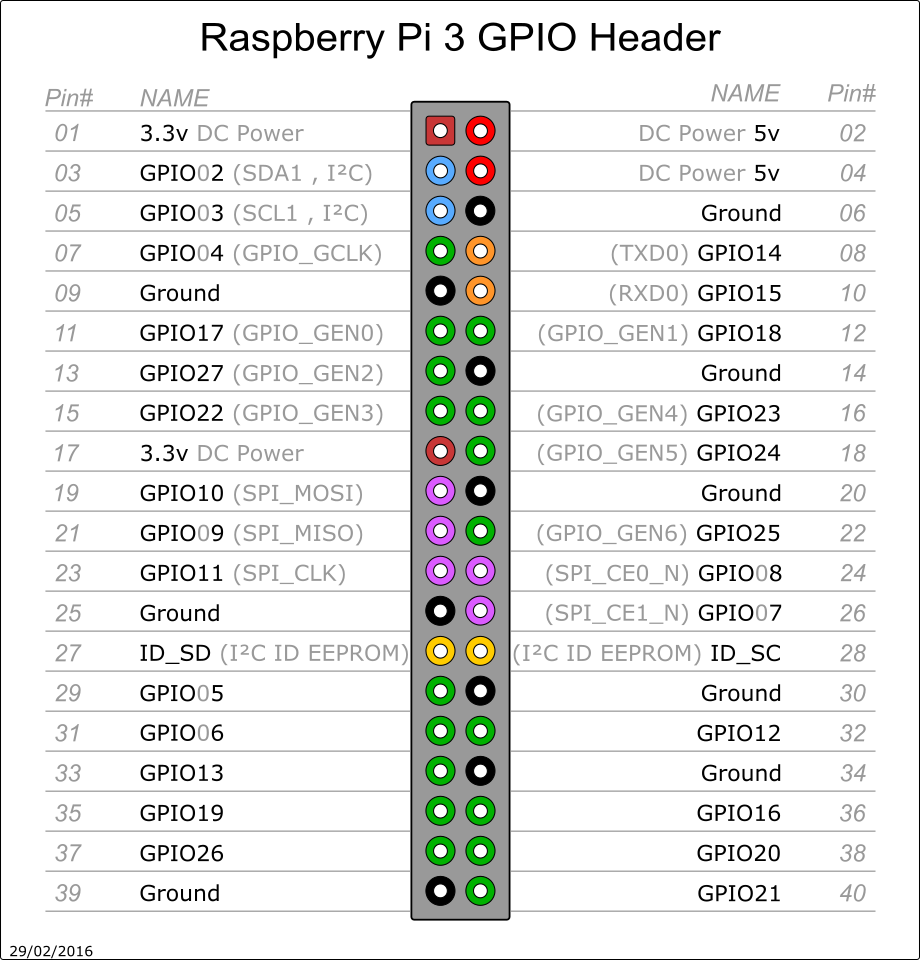
\includegraphics[scale=0.2]{images/gpiopinout.png}}
	\caption{Raspberry Pi 3 Model B GPIO Pinout Diagram (taken from  \cite{pigpiopinout})}
	\label{gpiopinout}
\end{figure} \newline  \noindent
In addition to simple GPIO functionality, some of the Raspberry Pi's GPIO pins have special functionality, like the ability to use serial communication making inter-device communication much easier. To send the number 1750 to an integrated circuit, the Raspberry Pi would need at least 11 free GPIO pins. While this is not impossible, the number of GPIO pins taken up by the single device is extremely inconvenient. This can easily be sent via serial connection with just two wires. Pins 3 and 5 can also be used to communicate with integrated circuits with the \(I^2 C\) protocol (Inter-Integrated Circuit). This allows bytes of data to be sent over only two wires \cite{backwhatisi2c}. This is done by \textit{serial communication}. Serial communication is where each bit of data (starting with the most significant bit, the highest value bit) is sent one after the other down a wire (the "data" line) \cite{backwhatisserpar} while another wire is used to synchronise the communication beteween devices (the "clock" line). Pins 19, 21, 23, 24, and 26 are used for another serial communications protocol, the Serial Peripherial Interface (SPI) protocol \cite{backwhatisspi}. SPI is similar to \(I^2 C\), although it differs in a few key ways.  \(I^2 C\) manages sub devices on the network using an address system which enables anything up to 128 devices connected together in one go, however SPI uses a simple select system where a signal is sent from a GPIO to the SPI device to tell it to expect instruction. This makes the SPI device far easier to work with, but less useful as the number of daisy-chained devices is limited by the number of free GPIO pins. \br
The high level languages used to create programs on desktop computers can be similarly used to write software on the Raspberry Pi. There are a number of software packages available for facilitating the communication with the GPIO pins. Built in to the Raspberry Pi are some basic packages, but for greater functionality third-party libraries are available for anyone to download and use\cite{pilibswiringpi, pilibspigpio}. The programming language "Python" is popular among software developers. Python is a high level, object oriented, interpreted language; making it well suited to quickly develop clean and easy to use software. Due to its popularity, Python has a vast number of packages available to perform any number of functions.

\section{Rheometry} % last edited 8/3/2017
The viscosity of a fluid is a measure of how resistant it is to flow. This is an important concept in process engineering: most processes involve fluids, many products are have fluid components. The viscosity (\(\mu\)) of a fluid can be calculated from the shear stress (\(\tau\)) imposed on a fluid and the rate at which it shears(\(\dot{\gamma}\)) using Newton's Law of Viscosity (Equation \ref{eqnvisco}) \cite{backfluidmech}.
\begin{equation}
\mu = \frac{\tau}{\dot{\gamma}}
\label{eqnvisco}
\end{equation}
There are different classes of fluids depending on how their viscosity behaves with respect to shear rate (the speed of the deformation) or the shear stress (the force behind the deformation). Newtonian fluids (like water) have a viscosity which is independent of the shear stress - proportional only to the shear rate. Some fluids have time-dependant viscosities: thixotropic fluids have a viscosity which apparently reduces the longer a stress is applied, and rheopectic fluids have a viscosity which apparently increases the longer a stress is applied. Other non-Newtonian fluids are dependant on the magnitude of the stress: shear-thinning fluids have a viscosity that appears to decrease with increased stress, and shear thickening fluids appear to experience a viscosity increase with an increase in stress \cite{backtypesofnonnewt}. Figures \ref{figshearthin} \& \ref{figshearthick} give examples of how shear rate varies with shear stress for non-Newtonian fluids. \br
\begin{figure}[!htb]
	\centering
	\fbox{
		\begin{subfigure}[t]{0.45\textwidth}
			\centering
			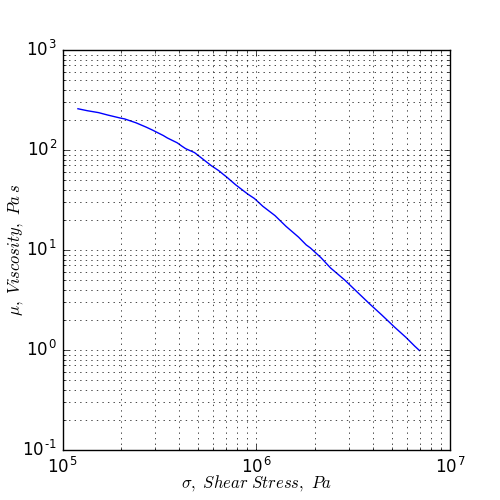
\includegraphics[scale=0.5]{figures/fig_shear_behav_thin.png}
			\caption{Shear Thinning}
			\label{figshearthin}
		\end{subfigure}
		\begin{subfigure}[t]{0.45\textwidth}
			\centering
			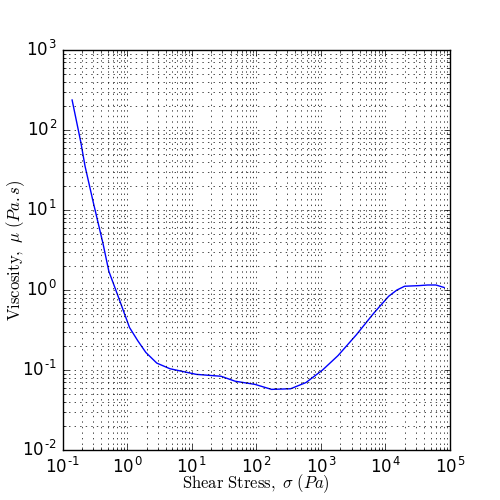
\includegraphics[scale=0.5]{figures/fig_shear_behav_thick.png}
			\caption{Shear Thickening}
			\label{figshearthick}
		\end{subfigure}
		%\fbox{\includegraphics[scale=0.25]{figures/fig_shear_behav.png}}
	}
	\label{figshearthinthick}
	\caption{Non-Newtonian Behaviour: Viscosity vs Shear Stress (adapted from \cite{figshearthin, figshearthick})}
\end{figure} %\newline  \noindent
Viscosity is measured in the lab using a rheometer. There are several distinct types of rheometers: capillary rheometers flow the fluid through a pipe of known dimensions and use the time taken to calculate the viscosity, cone-and-plate rheomters use a plate upon which is the fluid to be tested, and into the fluid is placed a cone which is spun (using the geometry and the torque/rotational rate of the spinning cone to calulate the viscosity), and the rotational rheometer which consists of a cylinder within another with the fluid to be tested between the cylinders such that it shears when a cylinder is rotated. \br
The capillary rheometer consists of a tube of known cross section, through which the test fluid is forced (by pumping, by piston). The viscosity can be found by measuring the flow rate and pressure gradient, and using the Hagen-Poiseulle equation for laminar flow through a pipe \cite{backcaprheom}. \cbh \br %(Information about the CR: how accurate can it be, what is it usually used for)
The cone-and-plate rheometer \cbh \br %(Information about the CAPR: how does it work, how accurate can it be, what is it usually used for)
The rotational rheometer is based upon the idea of couette flow: two infinitely long plates (separated by a known amount) between which is the fluid. In this scenario, \cbh
constructed from two cylinders: the outer (hollow) cylinder and the inner cylinder. The cylinders are positioned vertically close together to limit the amount of fluid shearing on the bottom of the inner cylinder.

\section{Colloidal Suspensions and Jamming} % last edited 8/3/2017
Fluids consisting of solid particles suspended in a liquid are prone to non-Newtonian behaviour, most commonly shear thinning (pseudoplastic). Some suspensions exhibit shear thickening behaviour, which has been explained in a number of ways. One theory explaining the onset of DST is the hydroclustering theory: as the suspension undergoes shear, the particles are forced together, forming larger particle groups. This increases the effective viscosity compared to low shear flow where the particles movements are not as restricted \cite[p.~7]{backbrownjaegrev}.
The order-disorder transition  theory explains the increase in viscosity as being due to an increase in stress causing the particles to become disordered. Initially there is a drop in viscosity, due to the particles in the suspension becoming more ordered. Then, as the stress is increased past a yield stress, the viscosity begins to increase due to a disruption in the order of the particles. % other theories?
\cbh \br
Shear thickening can be split further into continuous shear thickening (CST) and discontinuous shear thickening (DST, also termed dilatancy). CST is where the viscosity increases proportionally past a yield stress. However, with DST the viscosity suddenly (almost asymptotically) jumps upwards after a yield stress. DST has been associated with an apparent decrease in volume fraction of suspensions - hence its alternative name of dilatency. This effect also lends credence to the order-disorder-transition theory of shear thickening: you would expect the volume fraction to decrease (void fraction to increase) if the particles are going from a neat, ordered arrangement into extreme disorder \cite[p.~7]{backbrownjaegrev}. \cbh \br % cite!
DST is thought to be closely linked to the concept of jamming, which is \textit{"the conversion of a liquid system into a solid by imposed stress"} \cite{backhawjam}. Jamming is found in many different systems: in solids entering a hopper \cite{back2djam}, in pedestrians walking down a corridor \cite{backpedjam}, and in traffic \cite{backcarjam}. This can cause problems in processes: halting flow, damaging mixing equipment \cite{backshearjambertrand}. \br 
Volume fraction of the suspension mixture is an important property when looking at jamming. A suspension's volume fraction (\( \Phi \)) is the ratio of the volume of suspended particles to the volume of fluid in the suspension. For spherical particles, there is a maximum fraction. The closest packing that can occur (face-centred cubic) results in a particle volume fraction of \( \Phi = 0.74 \). However, at this packing the suspension is no longer a suspension and the particles are all in constant contact. The highest volume fraction of a suspension that still allows fluid to pass between the particles (particles are lubricated) is \( \Phi = 0.64 \) \cite{backguypoonjam}. As volume fraction increases, the likelihood of a suspension to undergo jamming increases (CITE). \br
Hard spheres is an approximation of the physical properties of the particles in a suspension. A "hard sphere" particle is a particle which is roughly spherical and with a fixed (non-intersectable) volume. \cbh \br
% "Normal" fluids (like water) exhibit Newtonian behaviour, this means that the rate of shear (how fast they deform) is directly proportional to the shear stress imposed upon them, with the constant of proportionality being the viscosity of the fluid\cite[p.~252]{schadict}. Multiphase suspensions can exhibit non-Newtonian viscous behaviour, where this direct relationship is not found \cite[p.~255-256]{schadict}. Some exhibit a shear-thickening behaviour: as the shear stress is increased, the shear rate decreases faster than in newtonian behaviour and others exhibit shear thinning .  Continuous shear thickening (shown in Figure \ref{figshearthick})  is an increase in the apparent viscosity. Discontinuous shear thickening is a sudden and extreme increase in the apparent viscosity of the fluid and is closely related to jamming, which is \textit{"the conversion of a liquid system into a solid by imposed stress"} \cite{backhawjam}. Jamming is found in many different systems: in solids entering a hopper \cite{back2djam}, in pedestrians walking down a corridor \cite{backpedjam}, and in traffic \cite{backcarjam}. This can cause problems in processes: halting flow, damaging mixing equipment \cite{backshearjambertrand}. \br	
%flow, shear, jam frequency %TODO
An interesting phenomenon that occurs in shearing suspensions is the formation and dissipation of "cracks" on the surface of the suspension. This can be directly seen in Figure \ref{cforscracks}. The cracks have been associated with a localized change in volume faction of the suspended particles \cite{backhawjam}. Another interesting optical property of jammed suspensions: the surface of a shear suspension has been found to alter texture, evidence of "Dilation" \cite{backbrownjaegrev}: caused by the particles in shear attempting to move around each other but having to take an inefficient route therefore decreasing the volume fraction of the suspension. This draws more fluid into the bulk and then the surface appears rough in texture, as opposed to glossy. 
\newline \newline \noindent
\begin{figure}[!htb]
	\centering
	\fbox{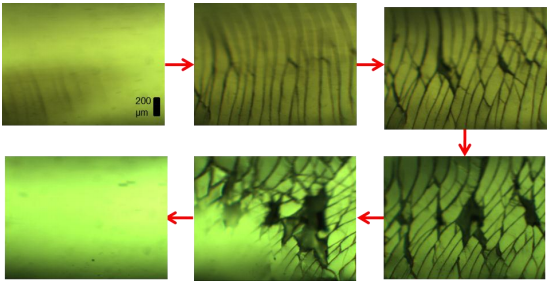
\includegraphics[scale=0.4]{images/cfors_cracks.png}}
	\caption{Suspension Surface Cracks (taken from \cite[p.~118]{thescforsyth})}
	\label{cforscracks}
\end{figure} \newline  \noindent


\section{This Project} % last edited 3/3/2017
This project aims to design, build, and test a control system for a bespoke jamming-focussed rheometer. \cbh
The experiment itself aims to gather more information about the statistical probability of the occurrence of a jam and how the shear stress affects this. \br
The experimental process consists of two concentric cylinders, the inner of which is attached to a DC motor and can be rotated. The gap between the two cylinders will be filled with a colloidal suspension. As the inner cylinder is rotated, the suspension will be subject to either a constant shear force, or a constant shear rate. 
%To find out how the formation of the cracks on the fluid's surface during shear correlate with the occurrence of discontinuous shear thickening, a camera will be aimed at the surface of the shearing fluid throughout the course of the experiment. The camera will be optically magnified using lenses placed in front of the aperture and will record images, which can later be processed using image recognition software to detect the formation of the cracks. \newline \newline \noindent
By knowing the power sent to the motor, as well as its efficiency and rotational speed, the strain rate and stress imposed upon the fluid in the rheomter can be calculated and thus used to obtain the rheology of the fluid - how the viscosity varies with time and stress. \br
The experimental set-up will be controlled by a Raspberry Pi 3 Model B. The Raspberry Pi's low cost, low power consumption, and GPIO availability make it a suitable choice for the controller to this process. Software will be developed for the Raspberry Pi to read in the motor's speed and the PEND's voltage reading, record it accurately and to control the rotational speed of the motor. In addition, the Raspberry Pi can be used to automate the experimental process by automatically altering experimental parameters in-between runs while logging all the relevant data during runs. The Pi can also be set up with a web interface, allowing monitoring of the experiment from remote locations, further reducing the manual workload on lab technicians. \br
Hardware was be developed to allow the Raspberry Pi to obtain the most accurate readings from the experiment as possible; the rotational speed of the motor, the electrical power supplied to the motor, the current shear stress observed within the fluid, and the presence of 'cracks' on the surface of the fluid.\br
Software will be developed to facilitate the accurate reading of information from the experiment, as well as control of the experimental parameters. There are two general operating modes; constant shear rate (or rotational speed), and constant shear stress (or torque). The former is relatively simple to do. By recording the motor's rotational speed and comparing with a set point, the speed can easily be held at a fixed point (thus a constant shear rate is achieved). The output torque is fixed in a similar way, using feedback from the process to fix the torque from the motor.


\end{document}